\documentclass[PdQ.tex]{subfiles}


\begin{document}

\hypertarget{\gl{PDCA}}{\section{PDCA}}

Il Plan-Do-Check-Act (PDCA), conosciuto anche come "Ciclo di Deming" o "Ciclo di miglioramento continuo", è un modello studiato per il miglioramento continuo della qualità in un’ottica a lungo raggio.\\ 
Questo modello permette di ricercare la qualità sui processi alla base del \gl{prodotto}, e non sul prodotto stesso.
Questo strumento permette di fissare degli obiettivi di miglioramento a partire dagli esiti delle misurazioni effettuate durante le varie attività di \gl{verifica}.
Una volta fissati gli obiettivi che si desiderano raggiungere, si iterano le quattro attività definite in seguito assicurando un incremento della qualità ad ogni ciclo.
\begin{figure}[htbp]
	\centering
	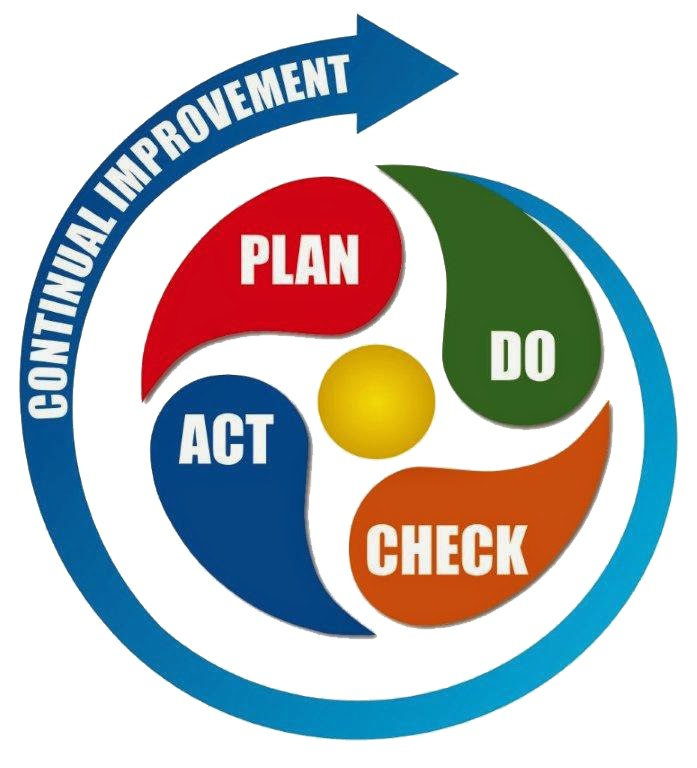
\includegraphics[height=6cm, width=5cm]{pdca.jpg}
	\caption{Continuous quality improvement with PDCA}\label{fig:pdca}
\end{figure}

\begin{itemize}
\item \textbf{Plan - Pianificare:} consiste nel definire gli obiettivi di miglioramento e le strategie da utilizzare per raggiungere la qualità attesa, in dettaglio:
\begin{itemize}
	\item identificare il problema o i processi da migliorare raccogliendo dati attraverso misurazioni;
	\item analizzare il problema in modo tale da capire quali sono gli effetti negativi definendone l'importanza e la priorità di intervento;
	\item definire gli obiettivi di massima in modo chiaro e quantitativo, indicando i benefici ottenibili con il suo raggiungimento. Devono essere definiti anche i tempi, gli indicatori e gli strumenti di controllo.
\end{itemize}
\item \textbf{Do - Eseguire:} consiste nell'esecuzione di ciò che è stato pianificato nel punto precedente e nella raccolta dati necessaria all'analisi effettuata nei punti successivi;
\item \textbf{ Check - Verificare:} consiste nel verificare l’esito del processo (per
efficienza ed efficacia) confrontandolo con i risultati attesi, così da poter definire se si va nella direzione giusta.  Vanno considerate metriche come la Schedule Variance e la completezza dei risultati attesi soddisfatti, vanno elaborati grafici e tabelle per avere una visione chiara di quanto rilevato. Una volta raggiunto l'obiettivo definito nella attività di Plan si può passare a quella di Act, mentre se questo non è soddisfatto è necessario ripetere un nuovo ciclo PDCA sullo stesso problema analizzando i vari stadi del ciclo precedente individuandone le cause del non raggiungimento dell’obiettivo stabilito;
\item \textbf{ Act - Agire:} si standardizza la soluzione individuata ed ogni membro del gruppo di lavoro viene formato e informato. Una volta terminato questo stadio si proseguirà nuovamente dallo stadio 1, con un nuovo problema.
\end{itemize}

Bisogna tener presente che se l’obiettivo è il miglioramento continuo, le attività devono essere analizzabili, ripetibili e tracciabili. Unendo queste tre caratteristiche è possibile individuare eventuali errori e correggerli.


\end{document}